\documentclass{beamer}
%Для защит онлайн лучше использовать разрешение 16x9
%\documentclass[aspectratio=169]{beamer}

\input{preamble.tex}

\usepackage{listings}
\usepackage{xcolor}
% Цвета для подсветки
\definecolor{json_key}{RGB}{0,128,128}     % Бирюзовый для двоеточий/ключей
\definecolor{json_string}{RGB}{42,0,255}   % Синий для строк
\definecolor{json_number}{RGB}{192,0,0}     % Темно-красный для чисел (по желанию)

\lstdefinelanguage{json}{
	string=[b]", % корректная обработка строк в кавычках
	stringstyle=\color{json_string}\ttfamily,
	% Заменяем только двоеточие, чтобы подсветить структуру, не трогая запятые и скобки
	literate=
	*{:}{{{\color{json_key}{:}}}}{1},
	% Если хотите, чтобы числа тоже подсвечивались, раскомментируйте строки ниже:
	%  {0}{{{\color{json_number}0}}}{1}
	%  {1}{{{\color{json_number}1}}}{1}
	%  {2}{{{\color{json_number}2}}}{1}
	%  {3}{{{\color{json_number}3}}}{1}
	%  {4}{{{\color{json_number}4}}}{1}
	%  {5}{{{\color{json_number}5}}}{1}
	%  {6}{{{\color{json_number}6}}}{1}
	%  {7}{{{\color{json_number}7}}}{1}
	%  {8}{{{\color{json_number}8}}}{1}
	%  {9}{{{\color{json_number}9}}}{1}
	%  {.}{{{\color{json_number}.}}}{1},
}

\lstset{
	basicstyle=\ttfamily\small,
	showstringspaces=false,
	breaklines=true,
	extendedchars=true, % важный параметр для поддержки спецсимволов и кириллицы
	literate={-}{{-}}1 % предотвращает превращение дефисов в длинные тире
}

\definecolor{codegreen}{rgb}{0,0.6,0}
\definecolor{codegray}{rgb}{0.5,0.5,0.5}
\definecolor{codepurple}{rgb}{0.58,0,0.82}
\definecolor{backcolour}{rgb}{0.95,0.95,0.92}

\lstdefinestyle{mystyle}{
	backgroundcolor=\color{backcolour},
	commentstyle=\color{codegreen},
	keywordstyle=\color{magenta},
	numberstyle=\tiny\color{codegray},
	stringstyle=\color{codepurple},
	basicstyle=\ttfamily\footnotesize,
	breakatwhitespace=false,
	breaklines=true,
	captionpos=b,
	keepspaces=true,
	numbers=left,
	numbersep=5pt,
	showspaces=false,
	showstringspaces=false,
	showtabs=false,
	tabsize=2
}

\usepackage{setspace}

\lstset{style=mystyle}

% То, что в квадратных скобках, отображается внизу по центру каждого слайда.
\title[Анализ MSD-сортировки]{Вероятностный апостериорный анализ трудоёмкости MSD-сортировки}

% То, что в квадратных скобках, отображается в левом нижнем углу.
\institute[СПбГУ]{}

% То, что в квадратных скобках, отображается в левом нижнем углу.
\author[Ерхов А. А.]{Ерхов Александр Александрович, группа 23.Б12-ПУ}

\begin{document}
{
\setbeamertemplate{footline}{}
% Лого университета или организации, отображается в шапке титульного листа
\begin{frame}
  
\includegraphics[width=1.4cm]{pictures/SPbGU_Logo.png}
\vspace{-35pt}
\hspace{-10pt}
\begin{center}
   \begin{tabular}{c}
        \scriptsize{Санкт-Петербургский государственный университет} \\
        \scriptsize{Кафедра компьютерных технологий и систем}
    \end{tabular}
\titlepage
\end{center}

\btVFill

{\scriptsize
  % У научного руководителя должна быть указана научная степень
   \textbf{Научный руководитель:} Никифоров Константин Аркадьевич, доцент кафедры моделирования электромеханических и компьютерных систем, кандидат физико-математических наук.
}
\begin{center}
  \vspace{5pt}
  \scriptsize{Санкт-Петербург\\
                 2026}
  \end{center}

\end{frame}
}

\begin{frame}[fragile]
  \frametitle{Введение}
  \textbf{Цель} -- провести апостериорный анализ трудоёмкости MSD-сортировки на основе результатов полученных в “A Limit Theorem for Radix Sort and Tries with Markovian Input” [1].
  \\ \textbf{Задачи:}
  \begin{itemize}
    \item Исследование материала [1].
    \item Разработка алгоритма на основе модели, приведенной в [1].
    \item Проведение вычислительного эксперимента.
    \item Проверка вхождения математического ожидания и дисперсии в соответствующие доверительные интервалы.
    \item Проверка центральной предельной теоремы c помощью критерия Пирсона.
  \end{itemize}
\end{frame}

\begin{frame}
  \frametitle{Постановка задачи}
  Будем рассматривать словарь (массив слов). Пусть алфавит $\Sigma = \{0, 1\}$. Количество символов в слове непостоянно. Количество слов в словаре также заранее не известно -- $n$.

  \textbf{Генерация словаря.} Каждое слово генерируется независимо друг от друга. Начальный символ, в каждом слове, выбирается согласно начальному распределению $\mu$, т. е. $P(\xi = 0) = \mu_0$, $P(\xi = 1) = \mu_1$, где $\mu_0+\mu_1=1$. Далее используем марковские цепи: каждый следующий символ зависит только от предыдущего, в соответствии с матрицей переходов $P = [p_{ij}], i, j \in \{0, 1\}$. При этом $p_{ij}\neq \dfrac{1}{2}, \forall i, j$ (Этот случай исключается как тривиальный). Также здесь введем понятие \textit{энтропии}:
  \begin{equation}
    H = \sum_i\pi_iH_i, \text{ где} \label{eq:H}
  \end{equation}
  \[
    H_i = - \sum_jp_{ij}\log p_{ij}, \pi_0=\dfrac{p_{10}}{p_{01}+p_{10}}, \pi_1 = \dfrac{p_{01}}{p_{01}+p_{10}}.
  \]
\end{frame}

\begin{frame}
  \frametitle{Априорный анализ}
  \begin{equation}
    \mathbb{E}[B_n^\mu] = \dfrac{1}{H}n\log n+O(n); \label{eq:E}
  \end{equation}
  \begin{equation}
    Var(B_n^\mu) = \sigma^2n\log n+O(n\sqrt{\log n}), \text{ где} \label{eq:Var}
  \end{equation}
  \[
    \begin{split}
          \sigma^2 = & \dfrac{\pi_0p_{00}p_{01}}{H^3}\left(\log(p_{00}/p_{01})+ \dfrac{H_1-H_0}{p_{01}+p_{10}}\right)^2 + \\
          & + \dfrac{\pi_1p_{10}p_{11}}{H^3}\left(\log(p_{10}/p_{11})+\dfrac{H_1-H_0}{p_{01}+p_{10}}\right)^2;
    \end{split}
  \]
  \begin{equation}
    \dfrac{B_n^\mu-\mathbb{E}[B_n^\mu]}{\sqrt{Var(B_n^\mu)}}  \stackrel{d}{\longrightarrow} \mathcal{N}(0,1) \label{eq:distribution}.
  \end{equation}
\end{frame}

\begin{frame}[fragile]
  \frametitle{Реализация}
  \begin{lstlisting}[language=Python]
  def MSD_sort(
      arr: list[str],
      n: int
  ) -> int:
    stack = [(0, 0, n)] # digit, left, right
    total_count = 0

    while stack:
      digit, left, right = stack.pop()
      if right-left <= 1 or digit >= max(len(arr[i]) for i in range(left, right)):
        continue
      count, groups = counting_sort(arr, left, right, digit)
      total_count += count
      for i in range(1, len(groups)):
        new_left, new_right = groups[i]
        if new_right - new_left > 1:
          stack.append((digit+1, new_left, new_right))

    return total_count
  \end{lstlisting}
\end{frame}

\begin{frame}
  \frametitle{Вычислительный эксперимент}
  $n = 10, 20, 40, ... 4096$ -- количество слов\\
  $k = 2n$ -- длинна слова\\
  $\Delta = n$ -- на столько может изменяться длинна слова ($k \pm \Delta$)\\
  $\mu = 0.7$ -- начальное распределение\\
  $P = [0.7, 0.2]$ -- матрица переходов\\
  $K = 60$ -- количество экспериментов для каждого $n$
\end{frame}

\begin{frame}
  \frametitle{Анализ}
  \begin{center}
    Для каждой выборки:\\
    \begin{doublespace}
      $\overline{X} = \dfrac{1}{K}\sum_{i=1}^{K}X_i$\\
      $S^2 = \dfrac{1}{K-1}\sum_{i=1}^{K}(X_i-\overline{X})^2$\\
      $\alpha = 0.05 \Rightarrow t_{crit} = 2.001$\\
      $CI = [\overline{X}-t_{crit}\dfrac{S}{\sqrt{K}}, \overline{X}+t_{crit}\dfrac{S}{\sqrt{K}}]$
    \end{doublespace}
    Нахождение констант:\\
    \begin{spacing}{2.5}
      $\nexists C: \dfrac{1}{H}n\log{n}+Cn \in CI, \forall n$\\
      $\exists C: \dfrac{2}{H}n\log{n}+Cn \in CI, \forall n$
    \end{spacing}
  \end{center}
\end{frame}

\begin{frame}
  \frametitle{Анализ}
  \begin{center}
    $\Delta = \overline{X} - \dfrac{1}{H}n\log{n}$\\
    \begin{figure}[h]
      \center{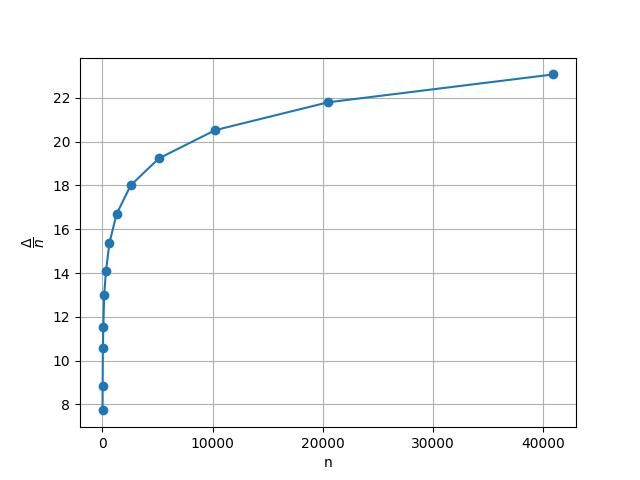
\includegraphics[width=0.7\linewidth]{pictures/Delta.png}}
      \caption{\label{img:Delta}График нормированных остатков}
    \end{figure}
  \end{center}
\end{frame}

\begin{frame}
  \frametitle{Дисперсия}
  \begin{onehalfspace}
      Так как по результату (\ref{eq:distribution}) наша случайная величина имеет нормальное распределение, то для проверки дисперсии имеет место $\chi^2$-интервал:
  \end{onehalfspace}
  \begin{spacing}{2.5}
    \begin{center}
      $CI = \left[\dfrac{(K-1)S^2}{\chi^2_{1-\alpha/2,K-1}}, \dfrac{(K-1)S^2}{\chi^2_{\alpha/2, K-1}}\right]$\\
      $\exists C: \sigma^2n\log{n}+Cn\sqrt{\log{n}}$
    \end{center}
  \end{spacing}
\end{frame}

\begin{frame}
  \frametitle{Исследование распределения}
  \begin{center}
    $K = \left(\dfrac{z_{1-\alpha/2}\sigma}{\delta}\right)^2$\\
    \begin{figure}[h]
      \center{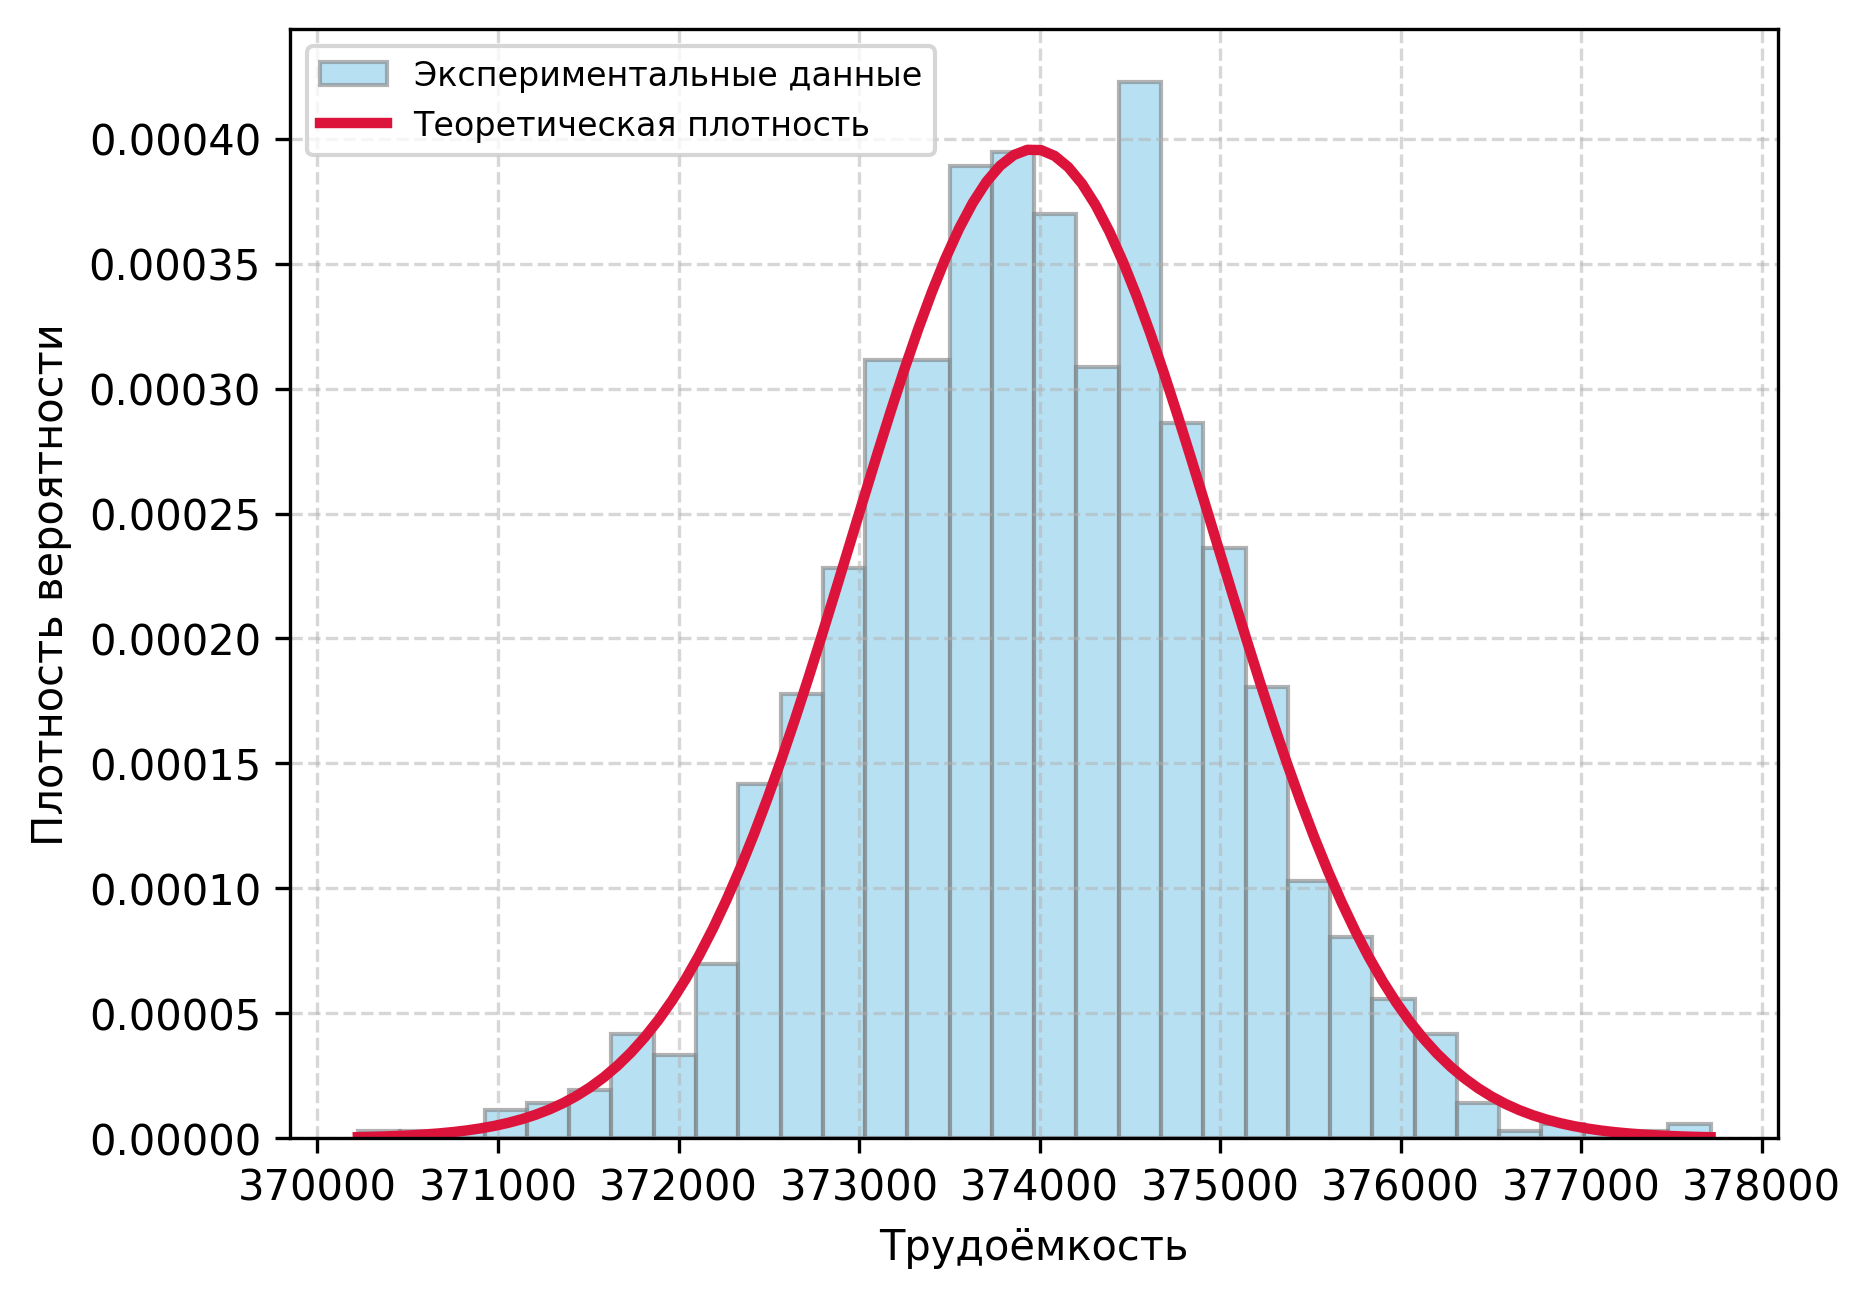
\includegraphics[width=0.6\linewidth]{pictures/freq.png}}
      \caption{\label{img:freq}Гистограмма частот}
    \end{figure}
    $b = 1 + \lfloor \log_2{K} \rfloor$
  \end{center}
\end{frame}

\begin{frame}
  \frametitle{Заключение}
  Поставленные в разделе \textit{Введение} цель и задачи выполнены. Вероятностная модель, описывающая поведение MSD-сортировки на данных, сгенерированных марковским источником, доказала свою точность. Алгоритм, несмотря на высокую трудоемкость в худшем случае, поддается строгому прогнозированию в среднем случае при известной матрице переходов алфавита.
\end{frame}

{
\setbeamertemplate{footline}{}
% Лого университета или организации, отображается в шапке титульного листа
\begin{frame}
  
\includegraphics[width=1.4cm]{pictures/SPbGU_Logo.png}
\vspace{-35pt}
\hspace{-10pt}
\begin{center}
   \begin{tabular}{c}
        \scriptsize{Санкт-Петербургский государственный университет} \\
        \scriptsize{Кафедра компьютерных технологий и систем}
    \end{tabular}
\titlepage
\end{center}

\btVFill

{\scriptsize
  % У научного руководителя должна быть указана научная степень
   \textbf{Научный руководитель:} Никифоров Константин Аркадьевич, доцент кафедры моделирования электромеханических и компьютерных систем, кандидат физико-математических наук.
}
\begin{center}
  \vspace{5pt}
  \scriptsize{Санкт-Петербург\\
                 2026}
  \end{center}

\end{frame}
}

\end{document}
